\documentclass{report}
\usepackage[pdftex]{graphicx}
\usepackage[english]{babel}
\usepackage{float}

\begin{document}
\title{Temperature Monitoring System}
\author{Mike Guzior, Jason Pearson, Marcel Englmaier and Justin Koehler}
\thanks{Client/Advisor: John Kapenga}
\maketitle
\tableofcontents
\newpage
\subsection*{Abstract}
\addcontentsline{toc}{subsection}{Abstract}
The goal of this project is to create an easy to use and low cost temperature monitoring system for anyone to use. 
The web end will allow the user to login in and view room statistics, as well as set warnings on thresholds. 
With the thresholds we would allow the user to select actions based on the threshold such as sending a text when it reaches a certain temperature. 
The room will contain a Raspberry Pi equipped with sensors which will use Ethernet to communicate to the web end and update information. 
The reason for using the Raspberry Pi’s is that we would be able to create a low cost sensor and be able to customize the code on the Pi as well. 
\newpage
\subsection*{Background}
\addcontentsline{toc}{subsection}{Background}
Our client has many needs that have been unmet for various reasons, with problems in their current situation, and our project provides solutions to those needs and provides resolutions to their problems.
\newline
\indent
Per Wikipedia, Western Michigan University's (WMU for short) Parkview campus was built in 2003 at a cost of $\$$72.5 million and is the home of the Western Michigan University College of Engineering and Applied Sciences (CEAS for short). 
 WMU’s engineering website explains that WMU has “state-of-the-art resources housed in a $\$$100 million high-tech facility”. 
Sadly, our client has advised that this did not include any automated temperature or humidity sensors and reporting equipment in any of the rooms. 
 These are absolutely critical in rooms that maintain computer, technology, manufacturing, and scientific equipment to safeguard the investment and resources of the university.
 Our client advised that there had been an incident where the temperature of servers increased unhindered to the point that equipment was destroyed due to this lack of automated environment reporting.
Since the fateful incident, WMU has had students implement several forms of reporting, and currently uses the Temperature @lert WiFi Edition to keep track of the temperature of rooms around campus. 
These sensors work very well but their major flaw is that they are very expensive. These sensors cost upwards of three hundred dollars per sensor and have many features that are neat, but unnecessary for our purposes. 
To alleviate this problem we proposed to create a server that would communicate with a network of home brewed, while reliable sensor computers. 
The server was created by another Western Michigan Computer Science senior design team and it currently is used to communicate with the @lert sensors.
\newline
\indent  
We are unaware at this time of some specific information regarding the facility such as the type and rating of their heating, ventilation, and air conditioning systems (HVAC for short), the dollar value of the equipment lost in the past, the british thermal units (BTU’s for short) that are generated by this equipment, or how fast the temperature would increase in the rare event of an HVAC malfunction, but it is clear that their need for automated reporting, and our solution will be more than adequate regardless of this information. 
It will increase autonomy, provide reporting, reduce cost, add better functionality, 
and provide a product that can be used by students and administrators a like.
\newline
\indent
	The currently used Temperature @lert WiFi sensor has accuracy of $\pm$.$5\,^{\circ}{\rm C}$. The max and minimum temperatures that the current sensor will calculate are -$10\,^{\circ}{\rm C}$ and +$85\,^{\circ}{\rm C}$. 
The current sensor also gives humidity readings. 
This is not high priority, but if we are able to implement it that would be desirable.
 The humidity readings that the current sensors give are between 10$\%$ and 90$\%$ relative humidity. 
This relative humidity has $\pm$ 3$\%$ relative humidity accuracy One major feature of the sensor is the fact that it can be used over the network using wired or wireless connections. 
The wireless specs that it abides by are the 802.11b/g standards and allow for WPA/WEP security. 
These are the features that are used by the system that we need to implement on our client devices.
\newline
\indent
The website that we inherited from the previous team initial page looks like the following figure. 
On this page it shows a graph of all the temperatures that are currently being tracked. 
This uses a framework that allows easy data viewing and little coding. 
We will probably use the same framework to impliment this graphing processs. 
Once logged in there is much more functionallity for the graphing. 
\begin{figure}[H]
\makebox[\textwidth]{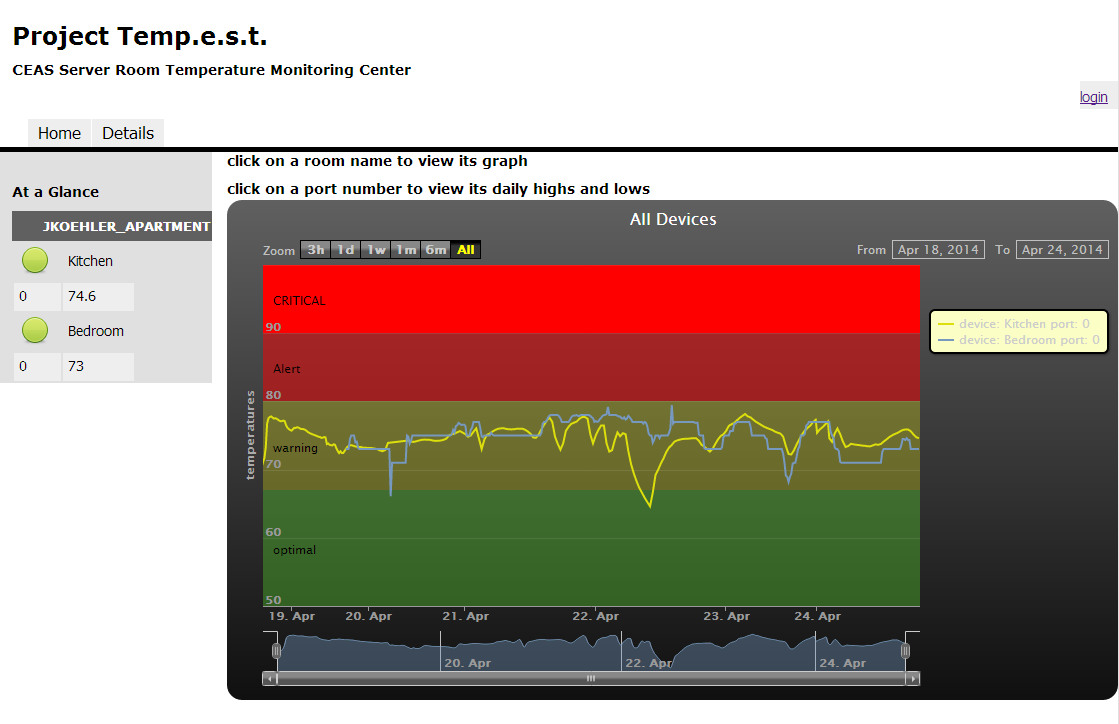
\includegraphics[width=\paperwidth]{Website.PNG}}
\caption{Initial View Of Site}
\end{figure}
\newpage
The login process is very basic at this time but in future release will utilize stricter security, data sanitization, and input verification,
and will prevent against session hijacking, network eavesdropping, cross site scripting, and brute force attacks. 
At this time the page will simply have a “Username” and “Password” field (along with a submit button) which will have functionality
added that disables the browser from remembering or saving this information. 
Our first “alpha” release will be using a test database with test users, test usernames, test passwords, and test data, so the security
will not be an issue during this phase. When the user submits, the framework will reference the data to see if it matches what is in the database, and if it does, provide further access to the site, and if not, it will require the user to try again. 
Session handling and potential cookies will be maintained by PHP sessions and session variables, which are handled by the CakePHP framework.
\newline
\indent
There will be only one login page, but based on whether the user successfully authenticates as an administrator or a simple user will determine the pages and views they have access to. 
The admin will have access to the identical pages as the user, but will have an administrator functionality added to the pages, which will allow them to add new users, rooms, and devices, as well as delete or modify existing users, rooms, and devices. 
A regular user will have a list of devices, whereas an administrator will see the same list but will have a button above said list that takes the to an “add device” page.  
The list will have an “edit” and “delete” button next to each device for administrators as well. The edit and delete pages will be similar to the add page, and will be basically the same for users, devices, and rooms. 
\begin{figure}[H]
\makebox[\textwidth]{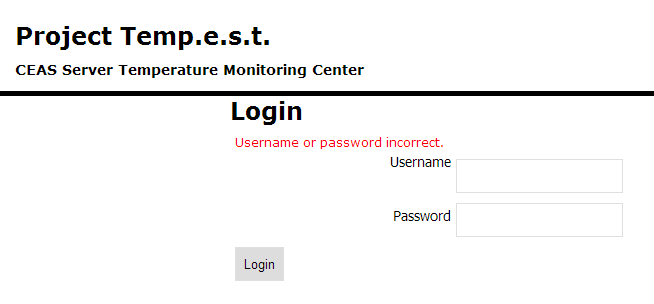
\includegraphics[width=\paperwidth]{LoginPage.PNG}}
\caption{Login Page}
\end{figure}
\newpage
The “Add” page will be basically the same for users, rooms, and devices. 
The page for users will have an empty form with fields appropriate for each user that includes UserID (in WMU’s case, it would be the WIN ID) FirstName, LastName, UserName, EmailAddress, and PhoneNumber. 
The Email and Phone fields will have a checkbox next to them that dictates whether that is a means of communication for alerts. 
The password is not an editable field, as it either (to be decided later) to be either randomly generated by the server, and required to have the user change it upon first login, 
or there will be an email verification process that allows the user to create their own password. 
Similarly for rooms and devices, appropriate fields will be listed and upon verification, will be added to the database. 
\begin{figure}[H]
\makebox[\textwidth]{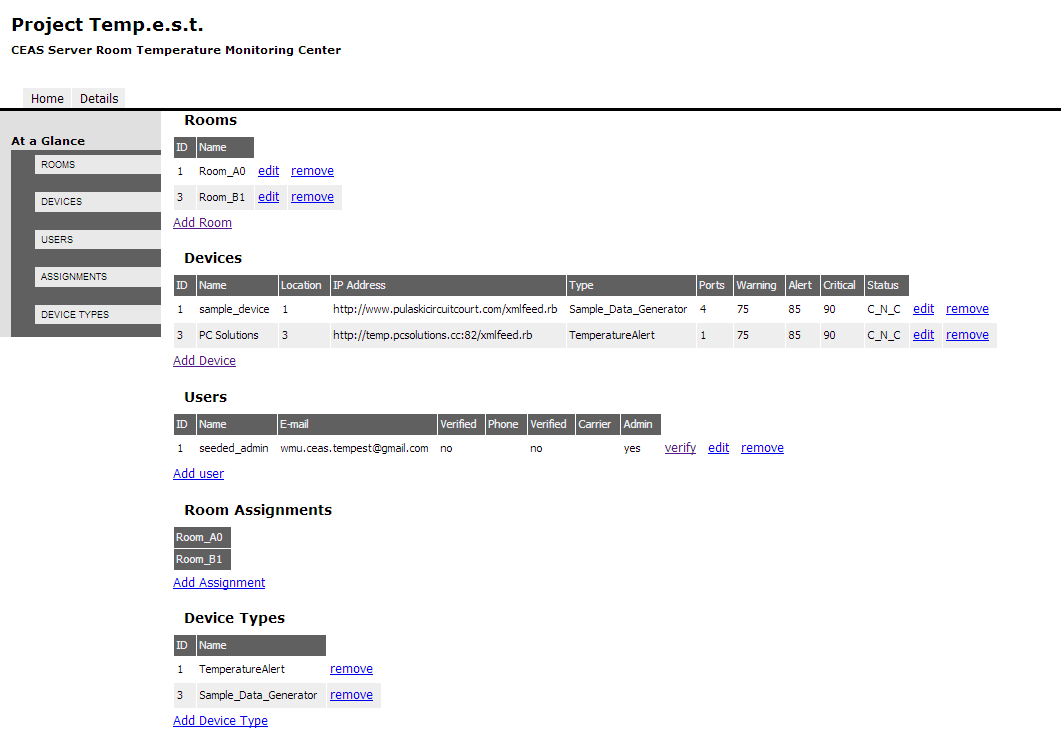
\includegraphics[width=\paperwidth]{AddPage.PNG}}
\caption{Add Page}
\end{figure}
\newpage

\begin{figure}[H]
\makebox[\textwidth]{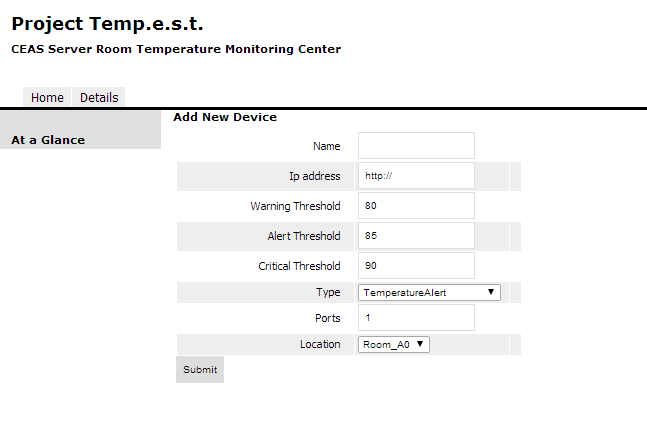
\includegraphics[width=\paperwidth]{AddDevice.PNG}}
\caption{Add Device To Network Page}
\end{figure}
This is the page that will be displayed when adding a new physical device to the network
\newpage

%\begin{figure}[H]
%\makebox[\textwidth]{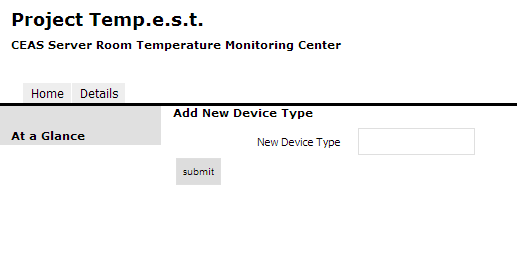
\includegraphics[width=\paperwidth]{AddDeviceType.PNG}}
%\caption{Add Another Device Type}
%\end{figure}
%\newpage
%	TODO: self explanitory
%
\begin{figure}[H]
\makebox[\textwidth]{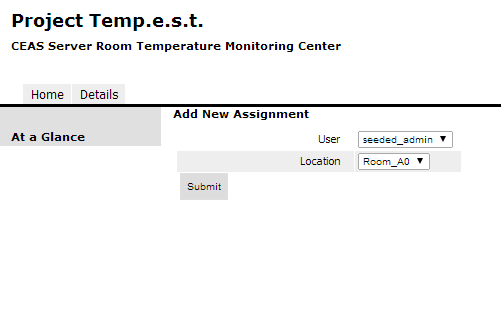
\includegraphics[width=\paperwidth]{AddRoomAssignment.PNG}}
\caption{Page to Assign Users to Rooms}
\end{figure}
Add an admin to oversee a server room
\newpage

\begin{figure}[H]
\makebox[\textwidth]{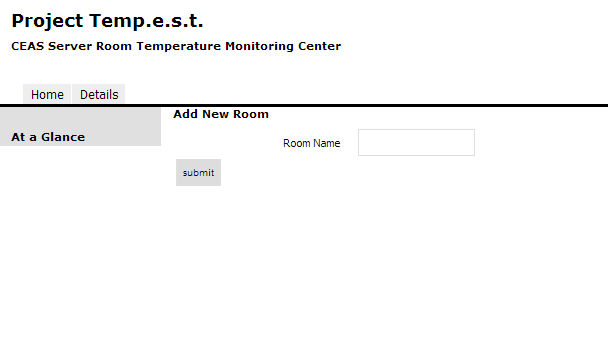
\includegraphics[width=\paperwidth]{AddRoom.PNG}}
\caption{Adds a Room}
\end{figure}
Add a server room to the list of rooms to monitor
\newpage

\begin{figure}[H]
\makebox[\textwidth]{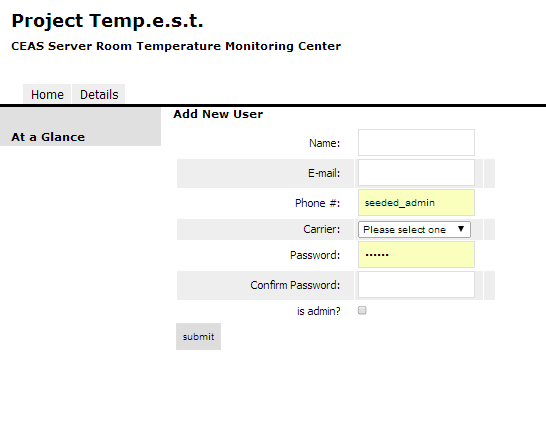
\includegraphics[width=\paperwidth]{AddUser.PNG}}
\caption{Page To Add Users}
\end{figure}
The page that will be displayed when adding a new user to the list of authorized admins
\newline
There will be three user levels
A main admin will be in cotrol of the whole system. Can add and remove users and middle admins, can see the entire system.
\newline
The middle admins will be able see the stats of the rooms they have access and will receive alerts for those rooms.
\newline
Users are only able to see the stats of each room. 
%\newpage <- Do we need this line?	

\newpage
\subsection*{Design Decisions}
\addcontentsline{toc}{subsection}{Design Decisions}
\begin{itemize}
\item Raspberry Pi: We decided to use the to connect to the temperature and humidity sensor because it is cost efficient and is able to send and receive data from the monitoring server. Other alternatives we looked at are the Arduino and the MSP430, but we ended up deciding on the raspberry pi because there was more documentation and had all the required hardware in one bundle.. Also Raspberry Pi’s require less hardware configuration allowing a end user with less hardware skills to still be able to utilize our project.
\item Git: Team members were more familiar with the workings of Git and could be used with a GUI.
\item Sensor: Team members spent a considerable amount of time exploring possible sensors, with the requirements being that the final solution utilize temperature and humidity sensing. As a single package, multiple solutions were found, but are currently too expensive to make them feasible. Much research was done into finding ones with Dallas One-Wire capability. One-Wire is a protocol which identifies each device separately, and can query each device using a single wire. Currently, only the DS18B20 temperature sensor is being used. A fitting humidity sensor for less that 5 dollars has not been found yet, but is still being looked for.
\item Cake PHP: We researched several languages to program our business logic and front end in, and we decided on PHP due to its high level
of portability, its ease of use, learning, and implementation, and its cost. 
The decision to use Cake PHP to rewrite the web application was made due to its very low learning curve in that it is written in PHP, for PHP, using the widely known design pattern of MVC. 
It is designed to be nearly identical to Microsoft’s .NET MVC 5 framework, so is easy to adapt to from anyone that primarily uses Microsoft technologies, and is written in PHP so anyone that utilizes open source technologies like PHP will have an easy time learning and using it as well. 
This project is designed to be accessible to anyone, so having this framework will be desirable by proponents of either closed or open source technologies. 
\end{itemize}
We have also decided to separate the project into 4 main functional pieces which each need their required spikes. The flow of the normal communication is as displayed as below.
TODO Fix the picture of the flow chart to meet the way that his laravell end was doing it
\newpage
\subsection*{Stories -- Requirements}
\addcontentsline{toc}{subsection}{Stories -- Requirements}
This project requires a server running linux, and in our case we will be using Ubuntu on this system. The project will also require a web server that runs any 2.x version of Apache, which according to W3Techs is used by 58.70$\%$ of all websites as of March 30th, 2014.  The choice to utilize Apache 2.x-compliant technologies was made with the idea that the majority of web servers utilize this technology, so it will be accessible to the majority. We also require a temperature sensor of your choice. We will be interfacing with two devices at first, beginning with the Temperature @lert WiFi edition TM-WIFI220, seen here:
\begin{figure}[H]
\makebox[\textwidth]{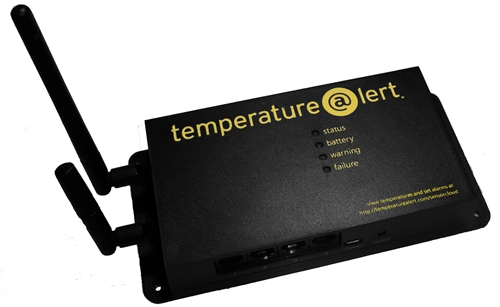
\includegraphics[width=\paperwidth]{AlertWiFi.PNG}}
\caption{@lert WiFi edition TM-WIFI220}
\end{figure}
 which has an initial cost of US $\$$300.00 +tax/shipping, a size footprint of H: 1.25”, W: 4.00”, L: 6.00”, an overall volume (excluding antennae) of 30 cubic inches, supports PoE, has a yearly estimated power usage of $\$$7.77 (based on 24 hour use @ $\$$0.1348 per kilowatt hour, and as is not able to by physically upgraded or added on to outside of its two available temperature and humidity sensors.
\newline
\indent
We are also designing our own sensing device that utilizes Raspberry Pi’s running rasberian, with a generic case it would appear as the following:
\begin{figure}[H]
\makebox[\textwidth]{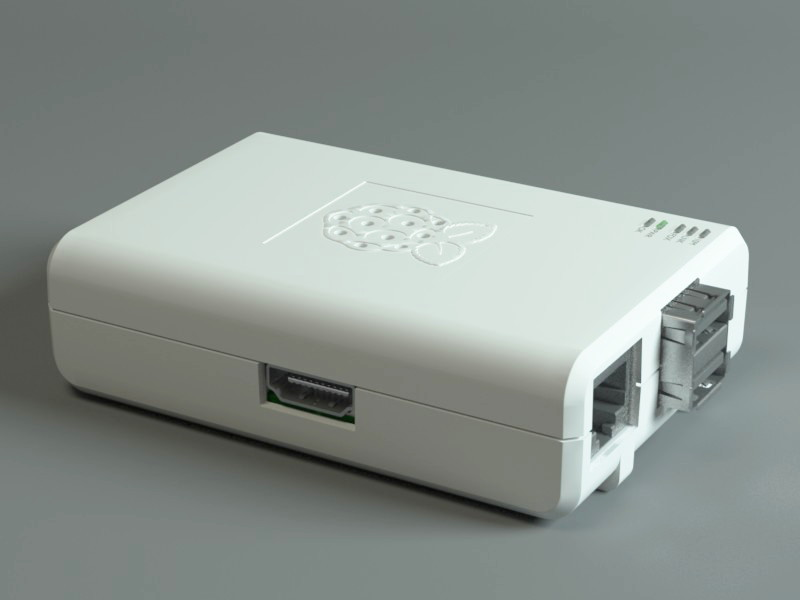
\includegraphics[width=\paperwidth]{Rasp.PNG}}
\caption{Example of Raspberry Pi}
\end{figure}
which has an initial cost of US $\$$61.47, a size footprint of H: 1.00”, W: 2.80”, L: 3.80”, an overall volume (excluding antennae) of 10.64 cubic inches, supports PoE, has a yearly estimated power usage of $\$$5.89 (based on 24 hour use @ $\$$0.1348 per kilowatt hour, and as is fully upgradeable in any capacity, with example sensors such as light sensors (for knowing if a windowless room has its lights on or off), motion sensors (to indicate movement in the room), video/still camera (for security monitoring), or even a touchscreen (for things like giving the unit the ability to edit settings without connecting to a computer, or using as an employee timeclock as an example), and the possibilities are endless.
. If you would like WiFi connectivity for your Raspberry Pi like we are going to, we will use a wireless receiver.
\newpage
\subsection*{Stories -- Functional}
\addcontentsline{toc}{subsection}{Stories -- Functional}
\begin {itemize}
\item Use a temperature sensor to monitor the temperature of the servers room located on the CEAS campus.
\item Check the humidity of the server rooms located on the CEAS campus.
\item Send the data to a server to be checked.
\item Use timers to make sure that communication with the servers are not lost
\item Send text messages and emails to the server administrators to alert them of loss of server connection and temperatures that are higher than the recommended level.
\item Establish permissions for the various admins that will be monitoring the system.
\end {itemize}
\newpage
\subsection*{Spikes}
\addcontentsline{toc}{subsection}{Spikes}
	To do these stories we will be creating spikes to show that critical sections are actually plausible. After we do this we combine the spikes and add minor code to complete the system. Some of our spikes are raspberry pi temperature retrieval code, raspberry to server communications, and sending emails to admins to name a few. 
\newpage
\subsection*{Resources}
\addcontentsline{toc}{subsection}{Resources}
\begin{itemize}
\item Raspberry Pi
\item Temperature Sensors
\item Humidity Sensors
\item Web Server
\item Soldering Equipment
\item Operating System loaded SD Cards with Rasperian
\item Power connectors for Raspberry pi
\item WiFi Connectors for Raspberry pi
\end{itemize}
\newpage
\subsection*{Feasibility}
\addcontentsline{toc}{subsection}{Feasibility}
Feasibility
	Based the cost of the hardware and the previous source code the feasibility of this project is high with many of the features being of low to mid risk. Extra features can be implemented very easily for future releases.
References
	For everything raspberry pi we use these sites
http://www.raspberrypi.org/
http://www.raspbian.org/
C Programming 2nd Edition
For everything web server these are the sites we use
	http://laravel.com/docs/quick
http://www.w3schools.com/
\newpage
\subsection*{Glossary}
\addcontentsline{toc}{subsection}{Glossary}
\begin{description}
\item [GUI] \hfill \\
Graphical User Interface. The windows a user interacts with.
\item [MSP430] \hfill \\
A 16-bit microcontroller platform made by Texas Instruments.
\item [Raspberry Pi] \hfill \\
 A credit-card-sized single-board computer developed by the Raspberry Pi Foundation.
\item [Arduino] \hfill \\
A series of microcontrollers that are very commonly used for computer to real world communications.
\item [Rasberian] \hfill \\
 A Debian based operating system that we will use for our Raspberry Pi’s
\item [CEAS] \hfill \\
College of Engineering and Applied Sciences at Western Michigan University.
\item [PHP] \hfill \\
A recursive acronym for “PHP Hypertext Preprocessor” - the web programming language being used.
\end{description}
\newpage
\subsection*{Ownership}
\addcontentsline{toc}{subsection}{OwnerShip}
\begin{description}
\item [Licenses] \hfill \\
Our project will be under several licenses. PHP is a free open source software released under the PHP Licensea.
CakePHP is licensed under the MIT license and per the agreement we are “free to modify, distribute and re-publish the source code on the condition that the copyright notices are left intact”.
In the event that our project was used to generate revenue, or be sold as a standalone software package, the license permits us “to incorporate CakePHP into any commercial or closed source application”.  
The GNU license and will be open source and will be hosted for all to access and modify as they desire on github.
\item [Intellectual Property (IP)] \hfill \\
As this project is being developed as a Senior Design project for Western Michigan University (WMU) at the direction of Dr. John Kapenga, WMU will retain the intellectual rights to the software.
\item [Non-Disclosure Agreement (NDA)] \hfill \\
No non-disclosure agreement is being used at this time.  The project is maintained on github, which is freely and openly accessible to anyone who wishes to view it, and is thus tracked by search engines such as Google, where it is able to be searched for by anyone on the planet.
\end{description}

\end{document}
